\documentclass[hyperref={pdfpagelabels=false}, xcolor=x11names,compress]{beamer}
\let\Tiny=\tiny
%% General document %%%%%%%%%%%%%%%%%%%%%%%%%%%%%%%%%%
\usepackage{tcolorbox}
\usepackage{color}
\usepackage{amsmath}

\usepackage{graphicx}


%% Beamer Layout %%%%%%%%%%%%%%%%%%%%%%%%%%%%%%%%%%
\useoutertheme[subsection=false,shadow]{miniframes}
\useinnertheme{default}
%\usefonttheme{serif}
%\usepackage{palatino}

\setbeamertemplate{navigation symbols}{}
\setbeamercovered{transparent = 0}

\setbeamerfont{title like}{shape=\scshape}
\setbeamerfont{frametitle}{shape=\scshape}

\definecolor{airforceblue}{rgb}{0.36, 0.54, 0.66}
\definecolor{aurometalsaurus}{rgb}{0.43, 0.5, 0.5}
\definecolor{midnightblue}{rgb}{0.1, 0.1, 0.44}
\definecolor{aqua}{rgb}{0.0, 1.0, 1.0}
\definecolor{darkgreen}{rgb}{0.0, 0.5, 0.0}

\setbeamercolor*{lower separation line head}{bg=airforceblue} 
\setbeamercolor*{normal text}{fg=black,bg=white} 
%\setbeamercolor*{alerted text}{fg=\definecolor{midnightblue}{rgb}{0.36, 0.54, 0.66}} 
\setbeamercolor*{example text}{fg=black} 
\setbeamercolor*{structure}{fg=black} 
 
\setbeamercolor*{palette tertiary}{fg=black,bg=black!10} 
\setbeamercolor*{palette quaternary}{fg=black,bg=black!10} 

\newcommand{\shownext}[1]{\onslide<+->{#1}}

\DeclareMathOperator*{\argmin}{arg\,min}

\newcommand{\<}[1]{\begin{column}{#1}}
\renewcommand{\>}{\end{column}}


\begin{document}

\begin{frame}
\title{Snowplow Route Optimisation \\in Lappeenranta}
%\subtitle{}
\author{Team Lambda!}
\date{}
\titlepage
\end{frame}


\section{Problem description}
\begin{frame}{Motivation}
\begin{center}


 In Finland winter is long and hard. It is importat for people that roads are regulary cleand od snow. During heavy snow storms the snowfall within 24 hours can reach a few dozen centimeters. Therefore, snow plowing may have to be done from none up \\ 
 to a few times a day throughout winter.
 \end{center}
\end{frame}

\begin{frame}{Question is ... }
\begin{center}\textbf{
How to find the shortest path for snow plowing machine \\ 
in Lappenranta?} \\


\includegraphics[scale=.25]{map.png}
\end{center}

\end{frame}

\begin{frame}
\includegraphics[width = \textwidth]{Map_of_Graph.pdf}
\end{frame}

\begin{frame}
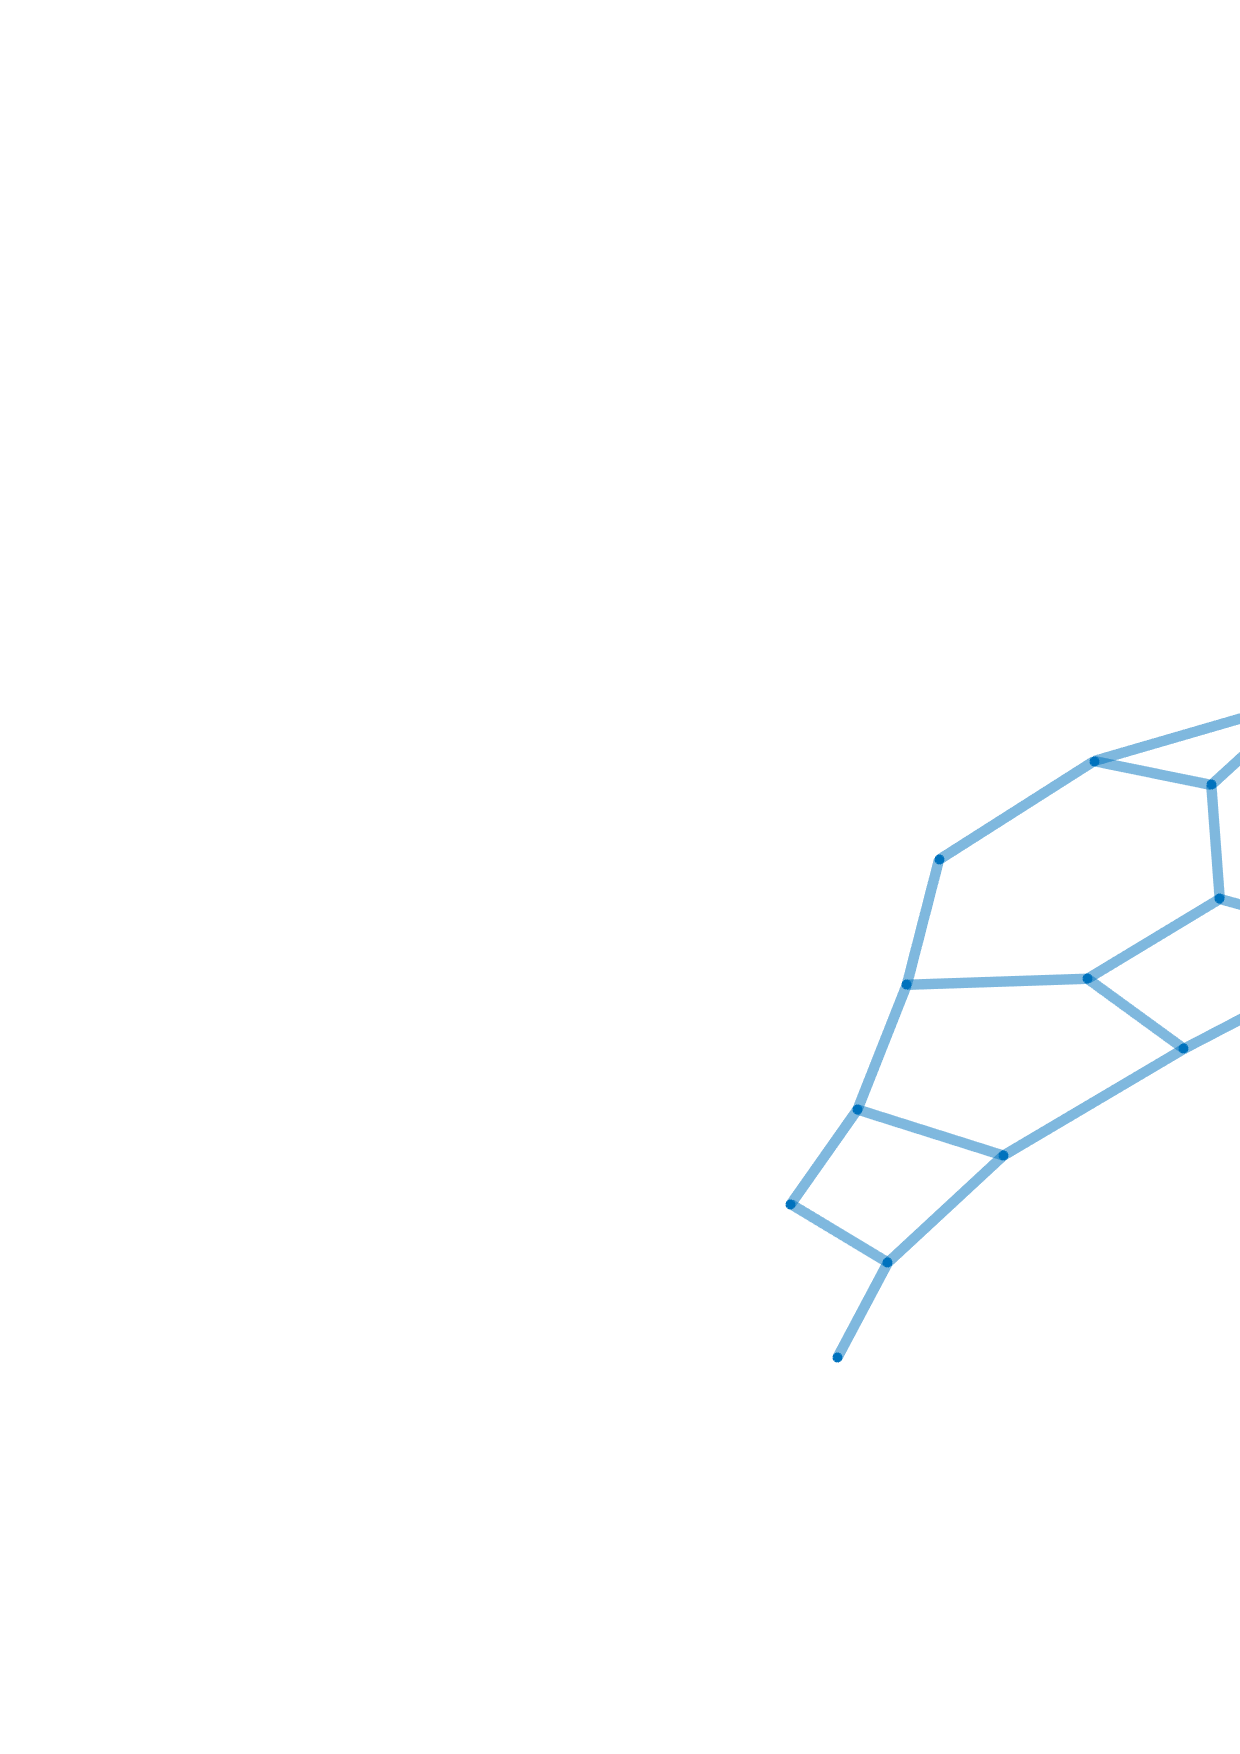
\includegraphics[width = \textwidth]{Lappeenranta_Graph.pdf}
\end{frame}

\end{document}